% -*- coding: utf-8 -*-

\begin{chapter}{Взаимодействие верхних слоев океана с ветром}\label{chap:9}
% \chapter{Response of the Upper Ocean to Winds}

Если вы когда то путешествовали вокруг Соединенных Штатов, то вы могли
заметить, что климат восточного побережья сильно отличается от климата
восточного побережья. Почему? Почему климат Чарльстона, Южная Каролина
так отличается от климата в Сан Диего, хотя оба они находятся
приблизительно на \latlon{32}{N} и оба недалеко от окена? В Чарльстоне
выпадает примерно $125$--$150\mm$ осадков ежегодно - в Сан Диего
$25$--$50$, в Чарльстоне летом жарко, в Сан Диего наоборот
прохладно. Или почему климат в Сан Франциско так отличен от климата
Норфолка, Вирджиния?
%
% If you have had a chance to travel around the United States, you may
% have noticed that the climate of the east coast differs considerably
% from that on the west coast. Why? Why is the climate of Charleston,
% South Carolina so different from that of San Diego, although both are
% near 32\degrees N, and both are on or near the ocean? Charleston has
% 125--150 cm of rain a year, San Diego has 25--50 cm, Charleston has
% hot summers, San Diego has cool summers. Or why is the climate of San
% Francisco so different from that of Norfolk, Virginia?

Если повнимательнее рассмотреть характеристики атмосферы вдоль двух
берегов около \latlon{32}{N}, то замечаются различия, которые могут
объяснить климат. Например, когда ветры с моря дуют прямо на Сан
Диего, они приносят слой прохладного, влажного морского воздуха
толщиной несколько сотен метров, над которым воздух намного суше и
теплее. В то же время, на восточном побережье, когда ветер дует с
моря, он приносит слой теплого влажного воздуха гораздо меньшей
толщины. Конвекция, которая является основной причиной возникновения
дождей, протекает гораздо активнее на восточном побережье, чем на
западном. Но почему слои воздуха над поверхностью воды так отличаются
на восточном и западном побережьях? Ответ может быть найден при
изучении взаимодействия океана с локальными ветрами, которые подробно
рассматриваются в этой главе.
%
% If we look closely at the characteristics of the atmosphere along the
% two coasts near 32\degrees N, we find more differences that may
% explain the climate. For example, when the wind blows onshore toward
% San Diego, it brings a cool, moist, marine, boundary layer a few
% hundred meters thick capped by much warmer, dry air. On the east
% coast, when the wind blows onshore, it brings a warm, moist, marine,
% boundary layer that is much thicker. Convection, which produces rain,
% is much easier on the east coast than on the west coast. Why then is
% the atmospheric boundary layer over the water so different on the two
% coasts? The answer can be found in part by studying the ocean's
% response to local winds, the subject of this chapter.

\begin{section}{Инерционное движение}
% \section{Inertial Motion}
Прежде, чем начать изучение течений около поверхности океана, давайте
обсудим простейшее решение уравнений движения, описывающих
взаимодействие океана и импульса, приводящего воду в
движение. Например, сильный ветер, дующий в течении нескольких часов,
приводит воду в движение и затем она движется только под воздействием
силы Кориолиса и силы тяготения. Никакие больше силы не действуют на
воду.
%
% \index{inertial!motion}To begin our study of currents near the sea
% surface, let's consider first a very simple solution to the equations
% of motion, the response of the ocean to an impulse that sets the water
% in motion.  For example, the impulse can be a strong wind blowing for
% a few hours. The water then moves only under the influence of Coriolis
% force. No other force acts on the water.

Такое движение называется движением по инерции. Если бы эта жидкость
была в невесомости, то она двигалась бы равномерно и прямолинейно,
согласно второму закону Ньютона. Но, к сожалению, из-за вращения Земли
движение ее выглядит совсем иначе.
%
% Such motion is said to be inertial. The mass of water continues to
% move due to its inertia. If the water were in space, it would move in
% a straight line according to Newton's second law. But on a rotating
% earth, the motion is much different.

Из (7.12) получаем уравнения движения идеальной жидкости:
\begin{subequations}
\begin{align}
 \frac{du}{dt}&=-\frac{1}{\rho}\,\frac{\partial{p}}{\partial{x}} + 2\Omega v\,\sin\varphi \\
 \frac{dv}{dt}&=-\frac{1}{\rho}\,\frac{\partial{p}}{\partial{y}} - 2\Omega u\,\sin\varphi \\
 \frac{dw}{dt}&=-\frac{1}{\rho}\,\frac{\partial{p}}{\partial{z}} + 2\Omega u\,\cos\varphi - g
\end{align}
\end{subequations}
Где $p$~--- давление, $\Omega = 2\,\pi$/(сидерический день) =
$7.292\times 10^{-5}\radps$~--- скорость вращения Земли вокруг своей
оси и $\varphi$~--- широта. Так же мы учитываем, что жидкость
идеальная(т.е. невязкая, $F_i = 0$).
%
% From (7.12) the equations of motion for a parcel of water moving in
% the ocean without friction are:
% \begin{subequations}
% \begin{align}
% \frac{du}{dt}&=-\frac{1}{\rho}\,\frac{\partial{p}}{\partial{x}} + 2\Omega v\,\sin\varphi \\
% \frac{dv}{dt}&=-\frac{1}{\rho}\,\frac{\partial{p}}{\partial{y}} - 2\Omega u\,\sin\varphi \\
% \frac{dw}{dt}&=-\frac{1}{\rho}\,\frac{\partial{p}}{\partial{z}} + 2\Omega u\,\cos\varphi - g
% \end{align}
% \end{subequations}
% where $p$ is pressure, $\Omega = 2\,\pi$/(sidereal day) $= 7.292
% \times 10^{-5}$ rad/s is the rotation of the earth in fixed
% coordinates, and $\varphi$ is latitude.

Теперь давайте искать простые решения этих уравнений. Чтобы это
сделать, мы должны упростить уравнения моментов. Итак, если только
гравитация и сила Кориолиса действуют на жидкость, то проекция
градиента давления на горизонтальную плоскость должна равняться нулю:
\begin{displaymath}
 \frac{\partial{p}}{\partial{x}} = \frac{\partial{p}}{\partial{y}} = 0
\end{displaymath}
Далее, мы можем предположить, что течение плоское, тогда система (9.1)
принимает вид:
\begin{subequations}
 \begin{align}
  \frac{du}{dt}&= 2\Omega \,v \sin\varphi =fv \\
  \frac{dv}{dt}&=-2\Omega \,u \sin\varphi = -fu
 \end{align}
\end{subequations}
где
\begin{equation}
 \boxed{f = 2\,\Omega\,\sin\varphi }
\end{equation}
есть параметр Кориолиса и $\Omega = 7.292 \times 10^{-5}\radps$~---
%% !!! в оригинале другая единица измерения, с^{-1}
скорость вращения Земли.
%
% Let's now look for simple solutions to these equations. To do this we
% must simplify the momentum equations. First, if only the Coriolis
% force acts on the water, there must be no horizontal pressure
% gradient:
% \begin{displaymath}
% \frac{\partial{p}}{\partial{x}} = \frac{\partial{p}}{\partial{y}} = 0
% \end{displaymath}
% Furthermore, we can assume that the flow is horizontal, and (9.1)
% becomes:
% \begin{subequations}
% \begin{align}
% \frac{du}{dt}&=2\Omega \,v \sin\varphi =fv \\
% \frac{dv}{dt}&=-2\Omega \,u \sin\varphi = -fu
% \end{align}
% \end{subequations}
% where:
% \begin{equation}
% \boxed{f = 2\,\Omega\,\sin\varphi }
% \end{equation}
% is the \textit{Coriolis Parameter}\index{Coriolis parameter|textbf}
% and $\Omega = 7.292 \times 10^{-5}$/s is the rotation rate of earth.

(9.2)~--- система линейных дифференциальных уравнений первого порядка,
 которая решается стандартными методами. Выразим~$u$ из второго
 уравнения и подставим в первое, получим:
\begin{displaymath}
 \frac{du}{dt}=-\frac{1}{f}\,\frac{d^2v}{dt^2}=fv
\end{displaymath}
Преобразуя правое равенство, получим уравнение гармонического
осциллятора:
\begin{equation}
 \frac{d^2v}{dt^2} + f^2v = 0
\end{equation}
решениями которого являются (9.5). Это течение называется инерциальным
течением или инерциальной осцилляцией:
\begin{equation}
\boxed{\begin{aligned}
u &= V\, \sin ft \\
v &= V\, \cos ft \\
V^2  &= u^2+v^2 \end{aligned}}
\end{equation}
Нужно отметить, что уравнения (9.5) являются параметрическим заданием
окружности диаметра $D_i = 2V/f$ и период 
$T_i = (2\pi)/f = T_{sd}/(2\sin\varphi)$ где
$T_{sd}$~--- сидерический день.
%
% Equations (9.2) are two coupled, first-order, linear, differential
% equations which can be solved with standard techniques. If we solve
% the second equation for $u$, and insert it into the first equation we
% obtain:
% \begin{displaymath}
% \frac{du}{dt}=-\frac{1}{f}\,\frac{d^2v}{dt^2}=fv
% \end{displaymath}
% Rearranging the equation puts it into a standard form we should
% recognize, the equation for the harmonic oscillator:
% \begin{equation}
% \frac{d^2v}{dt^2} + f^2v = 0
% \end{equation}
% which has the solution (9.5). This current is called an
% \textit{inertial current}\index{inertial!current|textbf} or
% \textit{inertial oscillation}\index{inertial!oscillation|textbf}:
% \begin{equation}
% \fbox{$ \D \begin{aligned}%{cc}
% u &= V\, \sin ft \\
% v &= V\, \cos ft \\
% V^2  &= u^2+v^2 \end{aligned}$}
% \end{equation}
% Note that (9.5) are the parametric equations for a circle with
% diameter $D_i = 2V/f$ and period $T_i = (2\pi)/f=
% T_{sd}/(2\sin\varphi)$ where $T_{sd}$ is a sidereal day.

\begin{figure}[t]
\makebox[120mm] [c]{\includegraphics{pics/inertialcur}}
\caption{Рис. 9.1 Инерционные течения на севере Тихого океана в
октябре 1987 (дни года 275-300) измерялись holey-sockdrifting buoy,
погруженным на 15м. Позиции проверялись 10-12 раз в день системой
Argos на метеорологическом спутнике NOAA. Наибольшее течение было
обнаружено на 277 день. И это не случайность. Вся поверхность
вращается. Буек, расположенный где угодно, показал бы схожий
результат. From van Meurs (1998).}
\label{fig:inertialcur}
\end{figure}
%
% \begin{figure}[t]
% \makebox[120mm] [c]{\includegraphics{inertialcur}}
% \footnotesize
% Figure 9.1 Inertial currents \rule{0mm}{3ex}in the North Pacific in
% October 1987 (days 275--300) measured by holey-sock drifting buoys
% drogued at a depth of 15 meters. Positions were observed 10--12 times
% per day by the Argos system\index{Argos system} on \textsc{noaa}
% polar-orbiting weather satellites and interpolated to positions every
% three hours. The largest currents were generated by a storm on day
% 277. Note these are not individual eddies. The entire surface is
% rotating. A drogue placed anywhere in the region would have the same
% circular motion. After van Meurs (1998).
% \label{fig:inertialcur}
% \vspace{-3ex}
% \end{figure}


$T_i$ is the inertial period, and it is one half the time required for
the rotation of a local plane on Earth's surface (Table 9.1). 
Направление вращения как у антициклона: по часовой стрелке в
северном полушарии и по часовой в южном. Инерционное течение~--- это
свободное движение масс воды на вращающейся плоскости.
%
% $T_i$ is the \textit{inertial
% period}\index{inertial!period|textbf}. It is one half the time
% required for the rotation of a local plane on earth's surface (Table
% 9.1). The rotation is
% \textit{anti-cyclonic}\index{anti-cyclonic|textbf}: clockwise in the
% northern hemisphere, counterclockwise in the southern. Inertial
% currents are the free motion of parcels of water on a rotating plane.

\begin{table}[h]
\caption{Инерционные осцилляции}
\begin{center}
\begin{tabular}{ccc}
\hline
Широта $(\varphi)$ & $T_i$ (ч) & $D$ (км) \\
                 & \multicolumn{2}{c}{для~$V = 20\cmps$} \\
\hline
$\degrees{90}$ & $11.97$ & $2.7$   \\
$\degrees{35}$ & $20.87$ & $4.8$   \\
$\degrees{10}$ & $68.93$ & $15.8$  \\
\hline
\end{tabular}
\end{center}
\end{table}
%
% \begin{table}[h!]\centering \small
% \vspace{-1ex}
% \begin{tabular*}{50mm}{@{}ccc@{}}
% \multicolumn{3}{@{}l@{}} {\bfseries Table 9.1 Inertial Oscillations} \\
% \hline
% Latitude $(\varphi)$ & $T_i$ (hr) & D\rule{0ex}{2.5ex} (km) \\
%                       & \multicolumn{2}{c}{for V = 20 cm/s} \\
% \hline
% 90\degrees & 11.97\rule{0ex}{2.5ex} & 2.7 \\
% 35\degrees & 20.87 & 4.8  \\
% 10\degrees & 68.93 & 15.8  \\ [0.5ex]
% \hline
% \end{tabular*} \\[0.5ex]
% \vspace{-3ex}
% \end{table}

Инерционные течения~--- наиболее распространенные течения в океане
(Рис. 9.1). Webster (1968) проанализировал много опубликованных работ
и обнаружил, что такие течения были обнаружены на всех глубинах и
широтах, но они непостоянны и затухают в течение нескольких
дней. Осцилляцияна различныхглубинах илиместах как правило непохожи.
%
% Inertial currents are the most common currents in the ocean (figure
% 9.1). Webster (1968) reviewed many published reports of inertial
% currents\index{inertial!current} and found that currents have been
% observed at all depths in the ocean and at all latitudes. The motions
% are transient and decay in a few days. Oscillations at different
% depths or at different nearby sites are usually incoherent.

Причиной возникновения инерционных течений является резкая смена ветра
у поверхности моря, так как она влечет за собой появление большой
осцилляции. Так же мы предполагали, что жидкость идеальная, когда
выписывали наши уравнения, но полностью пренебрегать вязкостью мы не
можем и через некоторое время осцилляция перейдет в другие
поверхностные течения.
%
% Inertial currents are caused by rapid changes of wind at the sea
% surface, with rapid changes of strong winds producing the largest
% oscillations. Although we have derived the equations for the
% oscillation assuming frictionless flow, friction cannot be completely
% neglected. With time, the oscillations decay into other surface
% currents. (See, for example, Apel, 1987: \S6.3 for more information.)
\end{section}

\begin{section}{Ekman Layer at the Sea Surface}
% \section{Ekman Layer at the Sea Surface}
Steady winds \index{Ekman layer|(}blowing on \index{Ekman layer!sea
surface|(}(the sea surface produce a thin, horizontal boundary layer,
the \textit{Ekman layer}. \index{Ekman layer!defined|textbf} By thin,
I mean a layer that is at most a few-hundred meters thick, which is
thin compared with the depth of the water in the deep ocean. A similar
boundary layer exists at the bottom of the ocean, the \textit{bottom
Ekman layer}\index{Ekman layer!bottom|textbf}, and at the bottom of
the atmosphere just above the sea surface, the planetary boundary
layer or frictional layer described in \S 4.3. The Ekman layer is
named after Professor Walfrid Ekman, who worked out its dynamics for
his doctoral thesis.
%
% Steady winds \index{Ekman layer|(}blowing on \index{Ekman layer!sea
% surface|(}(the sea surface produce a thin, horizontal boundary layer,
% the \textit{Ekman layer}. \index{Ekman layer!defined|textbf} By thin,
% I mean a layer that is at most a few-hundred meters thick, which is
% thin compared with the depth of the water in the deep ocean. A similar
% boundary layer exists at the bottom of the ocean, the \textit{bottom
% Ekman layer}\index{Ekman layer!bottom|textbf}, and at the bottom of
% the atmosphere just above the sea surface, the planetary boundary
% layer or frictional layer described in \S 4.3. The Ekman layer is
% named after Professor Walfrid Ekman, who worked out its dynamics for
% his doctoral thesis.

Ekman's work was the first of a remarkable series of studies conducted
during the first half of the twentieth century that led to an
understanding of how winds drive the ocean's circulation (Table
9.1). In this chapter we consider Nansen and Ekman's work. The rest of
the story is given in chapters 11 and 13.
%
% Ekman's work was the first of a remarkable series of studies conducted
% during the first half of the twentieth century that led to an
% understanding of how winds drive the ocean's circulation (Table
% 9.1). In this chapter we consider Nansen and Ekman's work. The rest of
% the story is given in chapters 11 and 13.

\begin{table}[t!]
\caption{Contributions to the Theory of the Wind-Driven Circulation}
\begin{tabular}{lcl}
\hline
Fridtjof Nansen     & (1898) 
  & Qualitative theory, currents transport water at an angle to the wind. \\
Vagn Walfrid Ekman  & (1902)    
  & Quantitative theory for wind-driven transport\index{transport!wind-driven} at 
    the sea surface. \\
Harald Sverdrup     & (1947)
  & Theory for wind-driven circulation in the eastern Pacific. \\
Henry Stommel   & (1948)     
  & Theory for westward intensification of wind-driven circulation 
    (western boundary currents). \\
Walter Munk  & (1950)
  & Quantitative theory for main features of the wind-driven circulation. \\
Kirk Bryan  & (1963)
  & Numerical models of the oceanic circulation. \\
Bert Semtner and Robert Chervin & (1988) 
  & Global, eddy-resolving, realistic model of the ocean's circulation. \\
\hline
\end{tabular}
\end{table}
%
% \begin{table}[t!]\small
% \begin{tabular*}{120mm}{@{}lcl@{}}
% \multicolumn{3}{@{}l@{}}{\bfseries Table 9.2 Contributions to the Theory of the
% \rule[-1ex]{0mm}{1ex}Wind-Driven Circulation}  \\
% \hline
% Fridtjof Nansen     & (1898)    & Qualitative \rule{0ex}{2.5ex}theory, currents transport water at an \\
% &&\hspace{1em}angle to the wind. \\
% Vagn Walfrid Ekman  & (1902)    & Quantitative theory for wind-driven
% transport\index{transport!wind-driven} at \\ &&\hspace{1em}the sea surface. \\
% Harald Sverdrup     & (1947)    & Theory for wind-driven circulation in the eastern \\
% &&\hspace{1em}Pacific. \\
% Henry Stommel   & (1948)     & Theory for westward intensification of wind-driven \\
% &&\hspace{1em}circulation (western boundary currents). \\
% Walter Munk  & (1950)   & Quantitative theory for main features of the wind- \\
% &&\hspace{1em}driven circulation. \\
% Kirk Bryan  & (1963)    & Numerical models of the oceanic circulation. \\
% Bert Semtner & (1988) & Global, eddy-resolving, realistic model of the \\
%  \ \ and Robert Chervin &&\hspace{1em}ocean's circulation. \\
% \hline
% \end{tabular*} \\[0.5ex]
% \vspace{-3ex}
% \end{table}

\begin{paragraph}{Nansen's Qualitative Arguments}
% \paragraph{Nansen's Qualitative Arguments}
Fridtjof Nansen noticed that wind tended to blow ice at an angle of
$\degrees{20}$--$\degrees{40}$ to the right of the wind in the Arctic, by
which he meant that the track of the iceberg was to the right of the
wind looking downwind (See figure 9.2). He later worked out the
balance of forces that must exist when wind tried to push icebergs
downwind on a rotating earth.
%
% Fridtjof Nansen noticed that wind tended to blow ice at an angle of
% 20\degrees--40\degrees\ to the right of the wind in the Arctic, by
% which he meant that the track of the iceberg was to the right of the
% wind looking downwind (See figure 9.2). He later worked out the
% balance of forces that must exist when wind tried to push icebergs
% downwind on a rotating earth.

Nansen argued that three forces must be important:
% Nansen argued that three forces must be important:
\begin{enumerate}
\item Wind Stress, \textbf{W};
%
% \vitem Wind Stress, \textbf{W};

\item 
Friction \textbf{F} (otherwise the iceberg would move as fast as the
wind);
%
% \vitem Friction \textbf{F} (otherwise the iceberg would move as fast
% as the wind);

\item 
Coriolis Force\index{Coriolis force}, \textbf{C}.
%
% \vitem Coriolis Force\index{Coriolis force}, \textbf{C}.
\end{enumerate}
Nansen argued further that the forces must have the following
attributes:
%
% Nansen argued further that the forces must have the following
% attributes:
\begin{enumerate}
\item 
Drag must be opposite the direction of the ice's velocity;
%
% \vitem Drag must be opposite the direction of the ice's velocity;

\item 
Coriolis force must be perpendicular to the velocity;
%
% \vitem Coriolis force must be perpendicular to the velocity;

\item 
The forces must balance for steady flow.  
%
% \vitem The forces must balance for steady flow.
\end{enumerate}
\begin{center}
\textbf{W} + \textbf{F} + \textbf{C} = 0
\end{center}
\end{paragraph}

\begin{paragraph}{Ekman's Solution}
% \paragraph{Ekman's Solution}
Nansen \index{Ekman layer!theory of}asked Vilhelm Bjerknes to let one
of Bjerknes' students make a theoretical study of the influence of
earth's rotation on wind-driven currents. Walfrid Ekman was chosen,
and he presented the results in his thesis at Uppsala (Kullenberg,
1954). Ekman later expanded the study to include the influence of
continents and differences of density of water (Ekman, 1905). The
following follows Ekman's line of reasoning in that paper.
%
% Nansen \index{Ekman layer!theory of}asked Vilhelm Bjerknes to let one
% of Bjerknes' students make a theoretical study of the influence of
% earth's rotation on wind-driven currents. Walfrid Ekman was chosen,
% and he presented the results in his thesis at Uppsala (Kullenberg,
% 1954). Ekman later expanded the study to include the influence of
% continents and differences of density of water (Ekman, 1905). The
% following follows Ekman's line of reasoning in that paper.

\begin{figure}[t!]
\centering
\makebox[120mm] [c]{\includegraphics{pics/forcesketch}}
\caption{The balance of forces acting on an iceberg in a wind on a rotating earth.}
\label{fig:forcesketch}
\vspace{-3ex}
\end{figure}
%
% \begin{figure}[t!]
% \centering
% \makebox[120mm] [c]{\includegraphics{forcesketch}}
% \footnotesize
% Figure 9.2 The balance of forces \rule{0mm}{3ex}acting on an iceberg
% in a wind on a rotating earth.
%
% \label{fig:forcesketch}
% \vspace{-3ex}
% \end{figure}

Ekman assumed\index{Ekman layer!Ekman's assumptions} a steady,
homogeneous, horizontal flow with friction on a rotating earth. Thus
horizontal and temporal derivatives are zero:
\begin{equation}
 \frac{\partial}{\partial{t}}=\frac{\partial}{\partial{x}}=\frac{\partial}{\partial{y}}=0
\end{equation}
For flow on a rotating earth, this leaves a balance between frictional
and Coriolis forces (8.15).  Ekman further assumed a constant vertical
eddy viscosity of the form (8:13):
\begin{equation}
 T_{xz} \,=\,\rho\, A_z \,\frac{\partial{u}}{\partial{z}}\: , \qquad 
 T_{yz} \,=\,\rho\, A_z \,\frac{\partial{v}}{\partial{z}}
\end{equation}
where $T_{xz}$, $T_{yz}$ are the components of the wind
stress\index{wind stress!components} in the $x$, $y$ directions, and
$\rho$ is the density of sea water.
%
% Ekman assumed\index{Ekman layer!Ekman's assumptions} a steady,
% homogeneous, horizontal flow with friction on a rotating earth. Thus
% horizontal and temporal derivatives are zero:
% \begin{equation}
% \frac{\partial}{\partial{t}}=\frac{\partial}{\partial{x}}=\frac{\partial}{\partial{y}}=0
% \end{equation}
% For flow on a rotating earth, this leaves a balance between frictional
% and Coriolis forces (8.15).  Ekman further assumed a constant vertical
% eddy viscosity of the form (8:13):
% \begin{equation}
% T_{xz} \,=\,\rho\, A_z \,\frac{\partial{u}}{\partial{z}}\: , \qquad T_{yz}\,=\,\rho\, A_z \,\frac{\partial{v}}{\partial{z}}
% \end{equation}
% where $T_{xz}$, $T_{yz}$ are the components of the wind
% stress\index{wind stress!components} in the $x$, $y$ directions, and
% $\rho$ is the density of sea water.

Using (9.7) in (8.15), the $x$ and $y$ momentum equations are:
\begin{subequations}
\begin{align}
fv +  A_z \, \frac{\partial{^2 u}}{\partial{z^2}} &= 0  \\
-fu + A_z \, \frac{\partial{^2 v}}{\partial{z^2}} &= 0
\end{align}
\end{subequations}
where $f$ is the Coriolis parameter\index{Coriolis parameter}.
%
% Using (9.7) in (8.15), the $x$ and $y$ momentum equations are:
% \begin{subequations}
% \begin{align}
% fv +  A_z \, \frac{\partial{^2 u}}{\partial{z^2}} &= 0  \\
% -fu + A_z \, \frac{\partial{^2 v}}{\partial{z^2}} &= 0
% \end{align}
% \end{subequations}
% where $f$ is the Coriolis parameter\index{Coriolis parameter}.

It is easy to verify that the equations (9.9) have solutions:
\begin{subequations}
\begin{align}
u &=  V_0\,\exp(az)\,\cos(\pi/4 + az)  \\
v &=  V_0\,\exp(az)\,\sin(\pi/4 + az)
\end{align}
\end{subequations}
when the wind is blowing to the north $(T = T_{yz})$. The constants
are
\begin{equation}
V_0 = \frac{T}{\sqrt{\rho^2_w\,f\,A_z}} \qquad \text{and} \qquad
a=\sqrt{\frac{f}{2A_z}}
\end{equation}
and $V_0$ is the velocity of the current at the sea surface.
%
% It is easy to verify that the equations (9.9) have solutions:
% \begin{subequations}
% \begin{align}
% u &=  V_0\,\exp(az)\,\cos(\pi/4 + az)  \\
% v &=  V_0\,\exp(az)\,\sin(\pi/4 + az)
% \end{align}
% \end{subequations}
% when the wind is blowing to the north $(T = T_{yz})$. The constants
% are
% \begin{equation}
% V_0 = \frac{T}{\sqrt{\rho^2_w\,f\,A_z}} \qquad \text{and} \qquad
% a=\sqrt{\frac{f}{2A_z}}
% \end{equation}
% and $V_0$ is the velocity of the current at the sea surface.

Now let's look at the form of the solutions. At the sea surface $z = 0$,
$\exp(z=0) = 1$, and
\begin{subequations}
\begin{align}
u(0) &= V_0\, \cos(\pi/4)  \\
v(0) &= V_0\, \sin(\pi/4)
\end{align}
\end{subequations}
The current has a speed of $V_0$ to the northeast. In general, the
surface current is $\degrees{45}$ to the right of the wind when looking
downwind in the northern hemisphere. The current is $\degrees{45}$ to the
left of the wind in the southern hemisphere. Below the surface, the
velocity decays exponentially with depth (figure 9.3):
\begin{equation}
\left[u^2(z) + v^2(z) \right]^{1/2} =V_0\,\exp(az)
\end{equation}
%
% Now let's look at the form of the solutions. At the sea surface $z = 0$,
% $\exp(z=0) = 1$, and
% \begin{subequations}
% \begin{align}
% u(0) &= V_0\, \cos(\pi/4)  \\
% v(0) &= V_0\, \sin(\pi/4)
% \end{align}
% \end{subequations}
% The current has a speed of $V_0$ to the northeast. In general, the
% surface current is 45\degrees\ to the right of the wind when looking
% downwind in the northern hemisphere. The current is 45\degrees\ to the
% left of the wind in the southern hemisphere. Below the surface, the
% velocity decays exponentially with depth (figure 9.3):
% \begin{equation}
% \left[u^2(z) + v^2(z) \right]^{1/2} =V_0\,\exp(az)
% \end{equation}

\begin{figure}[h!]
\makebox[121mm] [c]{\includegraphics{pics/ekmancurrent}}
\caption{Ekman current generated by a 10 m/s wind at \latlon{35}{N}.}
\label{fig:ekmancurrent}
\end{figure}
%
% \begin{figure}[h!]
% \makebox[121mm] [c]{\includegraphics{ekmancurrent}}
% \centering
% \footnotesize
% Figure 9.3. Ekman current \rule{0mm}{4ex}generated by a 10 m/s wind at
% 35\degrees\ N.
%
% \label{fig:ekmancurrent}
% \end{figure}
\end{paragraph}

\begin{paragraph}{Values for Ekman's Constants}
% \paragraph{Values for Ekman's Constants}
To proceed further, \index{Ekman layer!surface-layer constants}we need
values for any two of the free parameters: the velocity at the
surface, $V_0$; the coefficient of eddy viscosity, $A_z$; or the wind
stress\index{wind stress!and Ekman layer} $T$.
%
% To proceed further, \index{Ekman layer!surface-layer constants}we need
% values for any two of the free parameters: the velocity at the
% surface, $V_0$; the coefficient of eddy viscosity, $A_z$; or the wind
% stress\index{wind stress!and Ekman layer} $T$.

The wind stress\index{wind stress!and Ekman layer} is well known, and
Ekman used the bulk formula (4.2):
\begin{equation}
 T_{yz} = T = \rho_{air}\, C_D \,U_{10}^2
\end{equation}
where $\rho_{air}$ is the density of air, $C_D$ is the drag
coefficient\index{drag!coefficient}, and $U_{10}$ is the wind speed at
10 m above the sea. Ekman turned to the literature to obtain values
for $V_0$ as a function of wind speed. He found:
\begin{equation}
 V_0 = \frac{0.0127}{\sqrt{\sin|\varphi|}}\, U_{10}, 
  \qquad \qquad |\varphi|\ge 10
\end{equation}
%
% The wind stress\index{wind stress!and Ekman layer} is well known, and
% Ekman used the bulk formula (4.2):
% \begin{equation}
% T_{yz} = T = \rho_{air}\, C_D \,U_{10}^2
% \end{equation}
% where $\rho_{air}$ is the density of air, $C_D$ is the drag
% coefficient\index{drag!coefficient}, and $U_{10}$ is the wind speed at
% 10 m above the sea. Ekman turned to the literature to obtain values
% for $V_0$ as a function of wind speed. He found:
% \begin{equation}
% V_0 = \frac{0.0127}{\sqrt{\sin|\varphi|}}\, U_{10}, \qquad \qquad
% |\varphi|\ge 10
% \end{equation}

With this information, he could then calculate the velocity as a
function of depth knowing the wind speed $U_{10}$ and wind direction.
%
% With this information, he could then calculate the velocity as a
% function of depth knowing the wind speed $U_{10}$ and wind direction.
\end{paragraph}

\begin{paragraph}{Ekman Layer Depth}
% \paragraph{Ekman Layer Depth}
\index{Ekman layer!depth|textbf}The thickness of the Ekman layer is
arbitrary because the Ekman currents decrease exponentially with
depth. Ekman proposed that the thickness be the depth $D_E$ at which
the current velocity is opposite the velocity at the surface, which
occurs at a depth $D_E = \pi/a$, and the \textit{Ekman layer depth}
is:
\begin{equation}
 \boxed{D_E = \sqrt{\frac{2\pi^2\,A_z}{f}}}
\end{equation}
%
% \index{Ekman layer!depth|textbf}The thickness of the Ekman layer is
% arbitrary because the Ekman currents decrease exponentially with
% depth. Ekman proposed that the thickness be the depth $D_E$ at which
% the current velocity is opposite the velocity at the surface, which
% occurs at a depth $D_E = \pi/a$, and the \textit{Ekman layer depth}
% is:
% \begin{equation}
% \boxed{D_E = \sqrt{\frac{2\pi^2\,A_z}{f}}}
% \end{equation}

Using (9.13) in (9.10), dividing by $U_{10}$, and using (9.14) and
(9.15) gives:
\begin{equation}
 D_E = \frac{7.6}{\sqrt{\sin|\varphi|}}\, U_{10}
\end{equation}
in SI units. Wind in meters per second gives depth in meters. The
constant in (9.16) is based on $\rho = 1027 $ kg/m$^3$, $\rho_{air} =
1.25 $ kg/m$^3$, and Ekman's value of $C_D = 2.6 \times 10^{-3}$ for
the drag coefficient\index{drag!coefficient}.
%
% Using (9.13) in (9.10), dividing by $U_{10}$, and using (9.14) and
% (9.15) gives:
% \begin{equation}
% D_E = \frac{7.6}{\sqrt{\sin|\varphi|}}\, U_{10}
% \end{equation}
% in SI units. Wind in meters per second gives depth in meters. The
% constant in (9.16) is based on $\rho = 1027 $ kg/m$^3$, $\rho_{air} =
% 1.25 $ kg/m$^3$, and Ekman's value of $C_D = 2.6 \times 10^{-3}$ for
% the drag coefficient\index{drag!coefficient}.

Using (9.16) with typical winds, the depth of the Ekman layer varies
from about 45 to 300 meters (Table 9.3), and the velocity of the
surface current varies from 2.5\% to 1.1\% of the wind speed depending
on latitude\index{Ekman layer!sea surface|)}.
%
% Using (9.16) with typical winds, the depth of the Ekman layer varies
% from about 45 to 300 meters (Table 9.3), and the velocity of the
% surface current varies from 2.5\% to 1.1\% of the wind speed depending
% on latitude\index{Ekman layer!sea surface|)}.

\begin{table}[h!]
\caption{Typical Ekman Depths}
\begin{centering}
\begin{tabular}{c|cc}
\hline
               &\multicolumn{2}{c}{Latitude}      \\
U$_{10}$ [m/s]  & $\degrees{15}$      & $\degrees{45}$ \\
\hline
5              & 75  m & 45 m       \\
10             & 150 m & 90 m       \\
20             & 300 m & 180 m      \\
\hline
\end{tabular}
\end{centering}
\end{table}
%
% \begin{table}[h!]\small \centering
% \vspace{-1ex}
% \begin{tabular*}{60mm}{@{}c|cc}
% \multicolumn{3}{@{}c@{}}{\bfseries Table 9.3 Typical Ekman Depths \rule[-1ex]{0mm}{1ex}}  \\
% \hline
%                &\multicolumn{2}{c}{Latitude}      \\
% U$_{10}$ [m/s]  & 15\degrees          & 45\degrees \\
% \hline
% 5              & \rule{0ex}{3ex}75  m & 45 m       \\
% 10             &                150 m & 90 m       \\
% 20             &                300 m & 180 m      \\
% \hline
% \end{tabular*} \\[0.5ex]
% \vspace{-3ex}
% \end{table}
\end{paragraph}

\begin{paragraph}{The Ekman Number: Coriolis and Frictional Forces}
% \paragraph{The Ekman Number: Coriolis and Frictional Forces}
The depth of the Ekman layer is closely related to the depth at which
frictional force is equal to the Coriolis force\index{Coriolis force}
in the momentum equation (9.9). The Coriolis force is $f u$, and the
frictional force is $A_z \partial^2 U/\partial z^2$. The ratio of the
forces, which is non dimensional, is called the \textit{Ekman
Number}\index{Ekman Number|textbf} $E_z$:
\begin{displaymath}
 E_z= \frac{\text{Friction Force}}{\text{Coriolis Force}} 
    = \frac{A_z\frac{\partial^2u}{\partial{z^2}}}{fu} 
    = \frac{A_z\frac{u}{d^2}}{fu}
\end{displaymath}
\begin{equation}
 \boxed{E_z = \frac{A_z}{f\,d^2}}
\end{equation}
where we have approximated the terms using typical velocities $u$, and
typical depths $d$. The subscript $z$ is needed because the ocean is
stratified and mixing in the vertical is much less than mixing in the
horizontal. Note that as depth increases, friction becomes small, and
eventually, only the Coriolis force remains.
%
% The depth of the Ekman layer is closely related to the depth at which
% frictional force is equal to the Coriolis force\index{Coriolis force}
% in the momentum equation (9.9). The Coriolis force is $f u$, and the
% frictional force is $A_z \partial^2 U/\partial z^2$. The ratio of the
% forces, which is non dimensional, is called the \textit{Ekman
% Number}\index{Ekman Number|textbf} $E_z$:
% \begin{displaymath}
% E_z=\frac{\text{Friction Force}}{\text{Coriolis Force}} = \frac{\D A_z\frac{\D\partial^2u}{\partial{z^2}}}{fu} = \frac{\D A_z\frac{\D
% u}{\D d^2}}{\D fu}
% \end{displaymath}
% \begin{equation}
% \boxed{E_z = \frac{A_z}{f\,d^2}}
% \end{equation}
% where we have approximated the terms using typical velocities $u$, and
% typical depths $d$. The subscript $z$ is needed because the ocean is
% stratified and mixing in the vertical is much less than mixing in the
% horizontal. Note that as depth increases, friction becomes small, and
% eventually, only the Coriolis force remains.

Solving (9.17) for $d$ gives
\begin{equation}
 d = \sqrt{\frac{A_z}{fE_z}}
\end{equation}
which agrees with the functional form (9.15) proposed by
Ekman. Equating (9.18) and (9.15) requires $E_z = 1/(2\pi^2) = 0.05$
at the Ekman depth. Thus Ekman chose a depth at which frictional
forces are much smaller than the Coriolis force.
%
% Solving (9.17) for $d$ gives
% \begin{equation}
% d = \sqrt{\frac{A_z}{fE_z}}
% \end{equation}
% which agrees with the functional form (9.15) proposed by
% Ekman. Equating (9.18) and (9.15) requires $E_z = 1/(2\pi^2) = 0.05$
% at the Ekman depth. Thus Ekman chose a depth at which frictional
% forces are much smaller than the Coriolis force.
\end{paragraph}

\begin{paragraph}{Bottom Ekman Layer}
% \paragraph{Bottom Ekman Layer}
\index{Ekman layer!bottom}The Ekman layer at the bottom of the ocean
and the atmosphere differs from the layer at the ocean surface. The
solution for a bottom layer below a fluid with velocity $U$ in the
$x$-direction is:
\begin{subequations}
\begin{align}
u&=U[1 - \exp(-az)\,\cos\,az]  \\
v&=U\,\exp(-az)\,\sin\,az
\end{align}
\end{subequations}
The velocity goes to zero at the boundary, $u = v = 0$ at $z = 0$. The
direction of the flow close to the boundary is $\degrees{45}$ to the left
of the flow $U$ outside the boundary layer in the northern hemisphere,
and the direction of the flow rotates with distance above the boundary
(figure 9.4). The direction of rotation is anti\-cyclonic with
distance above the bottom.
%
% \index{Ekman layer!bottom}The Ekman layer at the bottom of the ocean
% and the atmosphere differs from the layer at the ocean surface. The
% solution for a bottom layer below a fluid with velocity $U$ in the
% $x$-direction is:
% \begin{subequations}
% \begin{align}
% u&=U[1 - \exp(-az)\,\cos\,az]  \\
% v&=U\,\exp(-az)\,\sin\,az
% \end{align}
% \end{subequations}
% The velocity goes to zero at the boundary, $u = v = 0$ at $z = 0$. The
% direction of the flow close to the boundary is 45\degrees\ to the left
% of the flow $U$ outside the boundary layer in the northern hemisphere,
% and the direction of the flow rotates with distance above the boundary
% (figure 9.4). The direction of rotation is anti\-cyclonic with
% distance above the bottom.

\begin{figure}[b!]
\makebox[121mm][c]{\includegraphics{pics/bottomekman}}
\caption{Ekman layer in the lowest kilometer of the
atmosphere (solid line), with wind velocity measured by Dobson (1914)
-\ -\ - \ . The numbers give height above the surface in meters. The
Ekman layer at the sea floor has a similar shape. After Houghton
(1977: 107).}
\end{figure}
%
% \begin{figure}[b!]
% \makebox[121mm] [c]{\includegraphics{bottomekman}}
% \footnotesize
% Figure 9.4 Ekman \rule{0mm}{3ex}layer in the lowest kilometer of the
% atmosphere (solid line), with wind velocity measured by Dobson (1914)
% -\ -\ - \ . The numbers give height above the surface in meters. The
% Ekman layer at the sea floor has a similar shape. After Houghton
% (1977: 107).
% \label{fig:bottomekman}
% %\vspace{-3ex}
% \end{figure}

Winds above the planetary boundary layer are perpendicular to the
pressure gradient in the atmosphere and parallel to lines of constant
surface pressure.  Winds at the surface are $\degrees{45}$ to the left
of the winds aloft, and surface currents are $\degrees{45}$ to the
right of the wind at the surface. Therefore we expect currents at the
sea surface to be nearly in the direction of winds above the planetary
boundary layer and parallel to lines of constant
pressure. Observations of surface drifters\index{drifters!in Pacific}
in the Pacific tend to confirm the hypothesis (figure 9.5).
%
% Winds above the planetary boundary layer are perpendicular to the
% pressure gradient in the atmosphere and parallel to lines of constant
% surface pressure.  Winds at the surface are 45\degrees\ to the left of
% the winds aloft, and surface currents are 45\degrees\ to the right of
% the wind at the surface. Therefore we expect currents at the sea
% surface to be nearly in the direction of winds above the planetary
% boundary layer and parallel to lines of constant
% pressure. Observations of surface drifters\index{drifters!in Pacific}
% in the Pacific tend to confirm the hypothesis (figure 9.5).

\begin{figure}[t!]
\makebox[121mm][c]{\includegraphics{pics/drifterplot}}
\caption{Trajectories of surface drifters\index{drifters!in Pacific}
in April 1978 together with surface pressure in the atmosphere
averaged for the month. Note that drifters tend to follow lines of
constant pressure except in the Kuroshio\index{Kuroshio!observed by
drifters} where ocean currents are fast compared with velocities in
the Ekman layer in the ocean. After McNally et al. (1983).}
\label{drifterplot}
\end{figure}
%
% \begin{figure}[t!]
% %\vspace{-2ex}
% \makebox[121mm] [c]{\includegraphics{drifterplot}}
% \footnotesize
% Figure 9.5 Trajectories \rule{0mm}{3ex}of surface
% drifters\index{drifters!in Pacific} in April 1978 together with
% surface pressure in the atmosphere averaged for the month. Note that
% drifters tend to follow lines of constant pressure except in the
% Kuroshio\index{Kuroshio!observed by drifters} where ocean currents are
% fast compared with velocities in the Ekman layer in the ocean. After
% McNally et al. (1983).
% \label{drifterplot}
% \vspace{-3ex}
% \end{figure}
\end{paragraph}

\begin{paragraph}{Examining Ekman's Assumptions}
% \paragraph{Examining Ekman's Assumptions}
Before \index{Ekman layer!Ekman's assumptions|(}considering the
validity of Ekman's theory for describing flow in the surface boundary
layer of the ocean, let's first examine the validity of Ekman's
assumptions. He assumed:
%
% Before \index{Ekman layer!Ekman's assumptions|(}considering the
% validity of Ekman's theory for describing flow in the surface boundary
% layer of the ocean, let's first examine the validity of Ekman's
% assumptions. He assumed:
%
\begin{enumerate}
\item 
No boundaries. This is valid away from coasts.
% \vitem No boundaries. This is valid away from coasts.

\item 
Deep water. This is valid if depth $\gg 200$ m.
% \vitem Deep water. This is valid if depth $\gg 200$ m.

\item 
$f$-plane. This is valid.
% \vitem $f$-plane. This is valid.

\item 
Steady state. This is valid if wind blows for longer than a pendulum
day.  Note however that Ekman also calculated a time-dependent
solution, as did Hasselmann (1970).
%
% \vitem Steady state. This is valid if wind blows for longer than a
% pendulum day.  Note however that Ekman also calculated a
% time-dependent solution, as did Hasselmann (1970).

\item $A_z$ is a function of $U^2_{10}$ only. It is assumed to be
independent of depth. This is not a good assumption. The mixed
layer\index{mixed layer!and Ekman layer} may be thinner than the Ekman
depth, and $A_z$ will change rapidly at the bottom of the mixed
layer\index{mixed layer!and Ekman layer} because mixing is a function
of stability. Mixing across a stable layer is much less than mixing
through a layer of a neutral stability. More realistic profiles for
the coefficient of eddy viscosity as a function of depth change the
shape of the calculated velocity profile. I reconsider this problem
below.
%
% \vitem $A_z$ is a function of $U^2_{10}$ only. It is assumed to be
% independent of depth. This is not a good assumption. The mixed
% layer\index{mixed layer!and Ekman layer} may be thinner than the Ekman
% depth, and $A_z$ will change rapidly at the bottom of the mixed
% layer\index{mixed layer!and Ekman layer} because mixing is a function
% of stability. Mixing across a stable layer is much less than mixing
% through a layer of a neutral stability. More realistic profiles for
% the coefficient of eddy viscosity as a function of depth change the
% shape of the calculated velocity profile. I reconsider this problem
% below.

\item 
Homogeneous density. This is probably good, except as it effects
stability.
%
% \vitem Homogeneous density. This is probably good, except as it
% effects stability.
\end{enumerate}\index{Ekman layer!Ekman's assumptions|)}
\end{paragraph}

\begin{paragraph}{Observations of Flow Near the Sea Surface}
% \paragraph{Observations of Flow Near the Sea Surface}
Does \index{Ekman layer!observations of}the flow close to the sea
surface agree with Ekman's theory? Measurements of currents made
during several, very careful experiments indicate that Ekman's theory
is remarkably good. The theory accurately describes the flow averaged
over many days.
%
% Does \index{Ekman layer!observations of}the flow close to the sea
% surface agree with Ekman's theory? Measurements of currents made
% during several, very careful experiments indicate that Ekman's theory
% is remarkably good. The theory accurately describes the flow averaged
% over many days.

Weller and Plueddmann (1996) measured currents from 2 m to 132 m using
14 vector-measuring current meters deployed from the Floating
Instrument Platform \textsc{flip} in February and March 1990 500 km
west of point Conception, California.  This was the last of a
remarkable series of experiments coordinated by Weller using
instruments on \textsc{flip}.
%
% Weller and Plueddmann (1996) measured currents from 2 m to 132 m using
% 14 vector-measuring current meters deployed from the Floating
% Instrument Platform \textsc{flip} in February and March 1990 500 km
% west of point Conception, California.  This was the last of a
% remarkable series of experiments coordinated by Weller using
% instruments on \textsc{flip}.

Davis, DeSzoeke, and Niiler (1981) measured currents from 2 m to 175 m
using 19 vector-measuring current meters deployed from a mooring for
19 days in August and September 1977 at \latlon{50}{N}, \latlon{145}{W} in
the northeast Pacific.
%
% Davis, DeSzoeke, and Niiler (1981) measured currents from 2 m to 175 m
% using 19 vector-measuring current meters deployed from a mooring for
% 19 days in August and September 1977 at 50\degrees N, 145\degrees W in
% the northeast Pacific.

Ralph and Niiler (2000) tracked 1503
drifters\index{drifters!measurement of Ekman currents} drogued to 15 m
depth in the Pacific from March 1987 to December 1994. Wind velocity
was obtained every 6 hours from the European Centre for Medium-Range
Weather Forecasts \textsc{ecmwf}.
%
% Ralph and Niiler (2000) tracked 1503
% drifters\index{drifters!measurement of Ekman currents} drogued to 15 m
% depth in the Pacific from March 1987 to December 1994. Wind velocity
% was obtained every 6 hours from the European Centre for Medium-Range
% Weather Forecasts \textsc{ecmwf}.

The results of the experiments indicate that:
% The results of the experiments indicate that:
\begin{enumerate}
\item
Inertial currents are the largest component of the flow.
% \vitem
% Inertial currents are the largest component of the flow.

\item 
The flow is nearly independent of depth within the mixed
layer\index{mixed layer!velocity within} for periods near the inertial
period\index{inertial!period}. Thus the mixed layer moves like a slab
at the inertial period. Current shear is concentrated at the top of
the thermocline\index{thermocline!and current shear}.
%
% \vitem 
% The flow is nearly independent of depth within the mixed
% layer\index{mixed layer!velocity within} for periods near the inertial
% period\index{inertial!period}. Thus the mixed layer moves like a slab
% at the inertial period. Current shear is concentrated at the top of
% the thermocline\index{thermocline!and current shear}.

\item 
The flow averaged over many inertial periods is almost exactly
that calculated from Ekman's theory. The shear of the Ekman currents
extends through the averaged mixed layer\index{mixed layer!and Ekman
layer} and into the thermocline. Ralph and Niiler found (using SI
units, $U$ in m/s):
\begin{align}
 D_E =& \frac{7.12}{\sqrt{\sin|\varphi|}}\, U_{10}\\
 V_0 =& \frac{0.0068}{\sqrt{\sin|\varphi|}}\, U_{10}
\end{align}
The Ekman-layer depth $D_E$ is almost exactly that proposed by Ekman
(9.16), but the surface current $V_0$ is half his value (9.14).
%
% \vitem 
% The flow averaged over many inertial periods is almost exactly
% that calculated from Ekman's theory. The shear of the Ekman currents
% extends through the averaged mixed layer\index{mixed layer!and Ekman
% layer} and into the thermocline. Ralph and Niiler found (using SI
% units, $U$ in m/s):
% \begin{align}
% D_E =& \frac{7.12}{\sqrt{\sin|\varphi|}}\, U_{10}\\
% V_0 =& \frac{0.0068}{\sqrt{\sin|\varphi|}}\, U_{10}
% \end{align}
% The Ekman-layer depth $D_E$ is almost exactly that proposed by Ekman
% (9.16), but the surface current $V_0$ is half his value (9.14).

\item 
The angle between the wind and the flow at the surface depends
on latitude, and it is near $\degrees{45}$ at mid latitudes (figure 9.6).
%
% \vitem 
% The angle between the wind and the flow at the surface depends
% on latitude, and it is near 45\degrees\ at mid latitudes (figure 9.6).

\item 
The transport is $\degrees{90}$ to the right
\index{transport!Ekman}of the wind in the northern hemisphere. The
transport direction agrees well with Ekman's theory.
%
% \vitem 
% The transport is 90\degrees\ to the right
% \index{transport!Ekman}of the wind in the northern hemisphere. The
% transport direction agrees well with Ekman's theory.
\end{enumerate}

\begin{figure}[t!]
\makebox[120mm][c]{\includegraphics{pics/ekmanangle}}
\caption{Angle between the wind and flow at the surface calculated by
Maximenko and Niiler using positions from drifters drogued at 15 m
with satellite-altimeter, gravity, and \textsc{grace}
\index{GRACE}data and winds from the \textsc{ncar/ncep} reanalysis.}
\label{fig:ekmanangle}
\end{figure}
%
% \begin{figure}[t!]
% %\vspace{-2ex}
% \makebox[120mm] [c]{\includegraphics{ekmanangle}}
% \footnotesize
% Figure 9.6 Angle \rule{0mm}{3ex}between the wind and flow at the
% surface calculated by Maximenko and Niiler using positions from
% drifters drogued at 15 m with satellite-altimeter, gravity, and
% \textsc{grace} \index{GRACE}data and winds from the \textsc{ncar/ncep}
% reanalysis.
% \label{fig:ekmanangle}
% \vspace{-3ex}
% \end{figure}
\end{paragraph}

\begin{paragraph}{Influence of Stability in the Ekman Layer}
% \paragraph{Influence of Stability in the Ekman Layer}
\index{Ekman layer!influence of stability}Ralph and Niiler (2000)
point out that Ekman's choice of an equation for surface currents
(9.14), which leads to (9.16), is consistent with theories that
include the influence of stability in the upper ocean.  Currents with
periods near the inertial period\index{inertial!period} produce shear
in the thermocline\index{thermocline!and current shear}. The shear
mixes the surface layers when the Richardson number falls below the
critical value (Pollard et al. 1973). This idea, when included in
mixed-layer theories, leads to a surface current $V_0$ that is
proportional to $\sqrt{N/f}$
\begin{equation}
 V_0 \sim U_{10}  \sqrt{N/f}
\end{equation}
where $N$ is the stability frequency defined by (8.36). Furthermore
\begin{equation}
 A_z \sim U_{10}^2 / N \qquad \text{and} \qquad D_E \sim U_{10} / \sqrt{Nf}
\end{equation}
Notice that (9.22) and (9.23) are now dimensionally correct. The
equations used earlier, (9.14), (9.16), (9.20), and (9.21) all
required a dimensional coefficient\index{Ekman layer|)}.
%
% \index{Ekman layer!influence of stability}Ralph and Niiler (2000)
% point out that Ekman's choice of an equation for surface currents
% (9.14), which leads to (9.16), is consistent with theories that
% include the influence of stability in the upper ocean.  Currents with
% periods near the inertial period\index{inertial!period} produce shear
% in the thermocline\index{thermocline!and current shear}. The shear
% mixes the surface layers when the Richardson number falls below the
% critical value (Pollard et al. 1973). This idea, when included in
% mixed-layer theories, leads to a surface current $V_0$ that is
% proportional to $\sqrt{N/f}$
% \begin{equation}
% V_0 \sim U_{10}  \sqrt{N/f}
% \end{equation}
% where $N$ is the stability frequency defined by (8.36). Furthermore
% \begin{equation}
% A_z \sim U_{10}^2 / N \qquad \text{and} \qquad D_E \sim U_{10} / \sqrt{Nf}
% \end{equation}
% Notice that (9.22) and (9.23) are now dimensionally correct. The
% equations used earlier, (9.14), (9.16), (9.20), and (9.21) all
% required a dimensional coefficient\index{Ekman layer|)}.
\end{paragraph}
\end{section}

\begin{section}{Ekman Mass Transport}
% \section{Ekman Mass Transport}
\index{Ekman transport!mass transport defined|textbf}
\index{transport!Ekman mass} \index{Ekman transport|(}Flow in the
Ekman layer at the sea surface carries mass. For many reasons we may
want to know the total mass transported in the layer. The
\textit{Ekman mass transport} $M_E$ is defined as the integral of the
Ekman velocity $U_E, V_E$ from the surface to a depth $d$ below the
Ekman layer. The two components of the transport are $M_{Ex}$,
$M_{Ey}$ :
\begin{equation}
 M_{Ex} = \int^0_{-d} \rho U_E \, dz, \qquad
 M_{Ey} = \int^0_{-d} \rho V_E \, dz
\end{equation}
The transport has units kg/(m$\cdot$s). It is the mass of water
passing through a vertical plane one meter wide that is perpendicular
to the transport and extending from the surface to depth $-d$ 
(figure 9.7).
%
% \index{Ekman transport!mass transport defined|textbf}
% \index{transport!Ekman mass} \index{Ekman transport|(}Flow in the
% Ekman layer at the sea surface carries mass. For many reasons we may
% want to know the total mass transported in the layer. The
% \textit{Ekman mass transport} $M_E$ is defined as the integral of the
% Ekman velocity $U_E, V_E$ from the surface to a depth $d$ below the
% Ekman layer. The two components of the transport are $M_{Ex}$,
% $M_{Ey}$ :
% \begin{equation}
% M_{Ex} = \int^0_{-d} \rho U_E \, dz, \qquad
% M_{Ey} = \int^0_{-d} \rho V_E \, dz
% \end{equation}
% The transport has units kg/(m$\cdot$s). It is the mass of water
% passing through a vertical plane one meter wide that is perpendicular
% to the transport and extending from the surface to depth $-d$ 
% (figure 9.7).

\begin{figure}[h!]
\makebox[120mm] [c]{\includegraphics{pics/transportsketch}}
\caption{Sketch for defining \textbf{Left:} mass
transports\index{transport!Ekman mass}, and \textbf{Right:} volume
transports\index{transport!Ekman volume}.}
\label{fig:transportsketch}
\end{figure}
%
% \begin{figure}[h!]
% \vspace{-2ex}
% \makebox[120mm] [c]{\includegraphics{transportsketch}}
% \centering
% \footnotesize
% Figure 9.7 Sketch for \rule{0mm}{3ex}defining \textbf{Left:} mass
% transports\index{transport!Ekman mass}, and \textbf{Right:} volume
% transports\index{transport!Ekman volume}.
% \label{fig:transportsketch}
% %\vspace{-1ex}
% \end{figure}

We calculate the Ekman mass transports\index{transport!Ekman} by
integrating (8.15) in (9.24):
\begin{align}
f\int_{-d}^0\rho\,V_E\,dz =f\,M_{Ey} &=-\int_{-d}^0 \,d T_{xz}   \notag \\
f\,M_{Ey} &=-T_{xz}\big|_{z=0} + T_{xz}\big|_{z=-d}
\end{align}
A few hundred meters below the surface the Ekman velocities approach
zero, and the last term of (9.25) is zero. Thus mass
transport\index{transport!Ekman mass} is due only to wind
stress\index{wind stress!and mass transport in ocean} at the sea
surface $(z = 0)$. In a similar way, we can calculate the transport in
the $x$ direction to obtain the two components of the \textit{Ekman
transport}:
\begin{subequations}
\begin{align}
f\,M_{Ey} &= -T_{xz}(0) \\
f\,M_{Ex} &= \;\;\; T_{yz}(0)
\end{align}
\end{subequations}
where $T_{xz}(0), T_{yz}(0)$ are the two components of the stress at
the sea surface.
%
% We calculate the Ekman mass transports\index{transport!Ekman} by
% integrating (8.15) in (9.24):
% \begin{align}
% f\int_{-d}^0\rho\,V_E\,dz =f\,M_{Ey} &=-\int_{-d}^0 \,d T_{xz}   \notag \\
% f\,M_{Ey} &=-T_{xz}\big|_{z=0} + T_{xz}\big|_{z=-d}
% \end{align}
% A few hundred meters below the surface the Ekman velocities approach
% zero, and the last term of (9.25) is zero. Thus mass
% transport\index{transport!Ekman mass} is due only to wind
% stress\index{wind stress!and mass transport in ocean} at the sea
% surface $(z = 0)$. In a similar way, we can calculate the transport in
% the $x$ direction to obtain the two components of the \textit{Ekman
% transport}:
% \begin{subequations}
% \begin{align}
% f\,M_{Ey} &= -T_{xz}(0) \\
% f\,M_{Ex} &= \;\;\; T_{yz}(0)
% \end{align}
% \end{subequations}
% where $T_{xz}(0), T_{yz}(0)$ are the two components of the stress at
% the sea surface.

Notice that the transport is perpendicular to the wind
stress\index{wind stress!and mass transport in ocean}, and to the
right of the wind in the northern hemisphere. If the wind is to the
north in the positive $y$ direction (a south wind), then $T_{xz}(0) =
0$, $M_{Ey} = 0$, and $M_{Ex} = T_{yz}(0)/f$. In the northern
hemisphere, $f$ is positive, and the mass transport is in the $x$
direction, to the east.
%
% Notice that the transport is perpendicular to the wind
% stress\index{wind stress!and mass transport in ocean}, and to the
% right of the wind in the northern hemisphere. If the wind is to the
% north in the positive $y$ direction (a south wind), then $T_{xz}(0) =
% 0$, $M_{Ey} = 0$, and $M_{Ex} = T_{yz}(0)/f$. In the northern
% hemisphere, $f$ is positive, and the mass transport is in the $x$
% direction, to the east.

It may seem strange that the drag of the wind on the water leads to a
current at right angles to the drag. The result follows from the
assumption that friction is confined to a thin surface boundary layer,
that it is zero in the interior of the ocean, and that the current is
in equilibrium with the wind so that it is no longer accelerating.
%
% It may seem strange that the drag of the wind on the water leads to a
% current at right angles to the drag. The result follows from the
% assumption that friction is confined to a thin surface boundary layer,
% that it is zero in the interior of the ocean, and that the current is
% in equilibrium with the wind so that it is no longer accelerating.

\textit{Volume transport}\index{Ekman transport!volume transport
defined|textbf}\index{transport!Ekman volume} $Q$ is the mass
transport divided by the density of water and multiplied by the width
perpendicular to the transport.
\begin{equation}
 Q_x=\frac{Y M_x}{\rho}, \qquad Q_y=\frac{X M_y}{\rho}
\end{equation}
where $Y$ is the north-south distance across which the eastward
transport\index{transport!eastward} $Q_x$ is calculated, and $X$ in
the east-west distance across which the northward transport $Q_y$ is
calculated. Volume transport has dimensions of cubic meters per
second. A convenient unit for volume transport in the ocean is a
million cubic meters per second. This unit is called a
\textit{Sverdrup}\index{Sverdrup|textbf}, and it is abbreviated Sv.
%
% \textit{Volume transport}\index{Ekman transport!volume transport
% defined|textbf}\index{transport!Ekman volume} $Q$ is the mass
% transport divided by the density of water and multiplied by the width
% perpendicular to the transport.
% \begin{equation}
% Q_x=\frac{Y M_x}{\rho}, \qquad Q_y=\frac{X M_y}{\rho}
% \end{equation}
% where $Y$ is the north-south distance across which the eastward
% transport\index{transport!eastward} $Q_x$ is calculated, and $X$ in
% the east-west distance across which the northward transport $Q_y$ is
% calculated. Volume transport has dimensions of cubic meters per
% second. A convenient unit for volume transport in the ocean is a
% million cubic meters per second. This unit is called a
% \textit{Sverdrup}\index{Sverdrup|textbf}, and it is abbreviated Sv.

Recent observations of Ekman transport \index{transport!Ekman,
observations of}in the ocean agree with the theoretical values
(9.26). Chereskin and Roemmich (1991) measured the Ekman volume
transport across \latlon{11}{N} in the Atlantic using an acoustic
Doppler current profiler described in Chapter 10. They calculated a
transport of $Q_y = 12.0 \pm 5.5$ Sv (northward) from direct
measurements of current, $Q_y = 8.8 \pm 1.9$ Sv from measured winds
using (9.26) and (9.27), and $Q_y = 13.5 \pm 0.3$ Sv from mean winds
averaged over many years at  \latlon{11}{N}.\index{Ekman transport|)}
%
% Recent observations of Ekman transport \index{transport!Ekman,
% observations of}in the ocean agree with the theoretical values
% (9.26). Chereskin and Roemmich (1991) measured the Ekman volume
% transport across 11\degrees N in the Atlantic using an acoustic
% Doppler current profiler described in Chapter 10. They calculated a
% transport of $Q_y = 12.0 \pm 5.5$ Sv (northward) from direct
% measurements of current, $Q_y = 8.8 \pm 1.9$ Sv from measured winds
% using (9.26) and (9.27), and $Q_y = 13.5 \pm 0.3$ Sv from mean winds
% averaged over many years at 11\degrees N.\index{Ekman transport|)}

\begin{paragraph}{Use of Transports}
% \paragraph{Use of Transports}
Mass \index{Ekman transport!uses}transports\index{transport!Ekman} are
widely used for two important reasons. First, the calculation is much
more robust than calculations of velocities in the Ekman layer. By
robust, I mean that the calculation is based on fewer assumptions, and
that the results are more likely to be correct. Thus the calculated
mass transport does not depend on knowing the distribution of velocity
in the Ekman layer or the eddy viscosity.
%
% Mass \index{Ekman transport!uses}transports\index{transport!Ekman} are
% widely used for two important reasons. First, the calculation is much
% more robust than calculations of velocities in the Ekman layer. By
% robust, I mean that the calculation is based on fewer assumptions, and
% that the results are more likely to be correct. Thus the calculated
% mass transport does not depend on knowing the distribution of velocity
% in the Ekman layer or the eddy viscosity.

Second, the variability of transport in space has important
consequences.  Let's look at a few applications.
%
% Second, the variability of transport in space has important
% consequences.  Let's look at a few applications.
\end{paragraph}
\end{section}

\begin{section}{Application of Ekman Theory}
% \section{Application of Ekman Theory}
Because steady winds blowing on the sea surface produce an Ekman layer
that transports \index{transport!and Ekman pumping}water at right
angles to the wind direction, any spatial variability of the wind, or
winds blowing along some coasts, can lead to
upwelling\index{upwelling!due to Ekman pumping}. And
upwelling\index{upwelling!importance of} is important:
%
% Because steady winds blowing on the sea surface produce an Ekman layer
% that transports \index{transport!and Ekman pumping}water at right
% angles to the wind direction, any spatial variability of the wind, or
% winds blowing along some coasts, can lead to
% upwelling\index{upwelling!due to Ekman pumping}. And
% upwelling\index{upwelling!importance of} is important:
%
\begin{enumerate}
\item 
Upwelling enhances biological productivity, which feeds fisheries.
%
% \vitem Upwelling enhances biological productivity, which feeds
% fisheries.

\item 
Cold upwelled water alters local weather. Weather onshore of regions
of upwelling\index{upwelling!and water temperature} tend to have fog,
low stratus clouds, a stable stratified atmosphere, little convection,
and little rain.
%
% \vitem Cold upwelled water alters local weather. Weather onshore of
% regions of upwelling\index{upwelling!and water temperature} tend to
% have fog, low stratus clouds, a stable stratified atmosphere, little
% convection, and little rain.

\item 
Spatial variability of transports in the open ocean leads to
upwelling\index{upwelling!due to Ekman pumping} and downwelling, which
leads to redistribution of mass in the ocean, which leads to
wind-driven geostrophic currents\index{geostrophic currents!and Ekman
pumping} via Ekman pumping\index{Ekman pumping}.
%
% \vitem Spatial variability of transports in the open ocean leads to
% upwelling\index{upwelling!due to Ekman pumping} and downwelling, which
% leads to redistribution of mass in the ocean, which leads to
% wind-driven geostrophic currents\index{geostrophic currents!and Ekman
% pumping} via Ekman pumping\index{Ekman pumping}.
\end{enumerate}

\begin{paragraph}{Coastal Upwelling}
% \paragraph{Coastal Upwelling}
To \index{Ekman layer!coastal upwelling}see how winds lead to
upwelling\index{upwelling!coastal}, consider north winds blowing
parallel to the California Coast (figure 9.8 left). The winds produce
a mass transport\index{transport!and upwelling} away from the shore
everywhere along the shore. The water pushed offshore can be replaced
only by water from below the Ekman layer. This is
\textit{upwelling}\index{upwelling|textbf} (figure 9.8 right). Because
the upwelled water is cold, the upwelling leads to a region of cold
water at the surface along the coast. Figure 10.16 shows the
distribution of cold water off the coast of California.
%
% To \index{Ekman layer!coastal upwelling}see how winds lead to
% upwelling\index{upwelling!coastal}, consider north winds blowing
% parallel to the California Coast (figure 9.8 left). The winds produce
% a mass transport\index{transport!and upwelling} away from the shore
% everywhere along the shore. The water pushed offshore can be replaced
% only by water from below the Ekman layer. This is
% \textit{upwelling}\index{upwelling|textbf} (figure 9.8 right). Because
% the upwelled water is cold, the upwelling leads to a region of cold
% water at the surface along the coast. Figure 10.16 shows the
% distribution of cold water off the coast of California.

\begin{figure}[t!]
\makebox[120mm][c]{\includegraphics{pics/upwelling}}
\caption{Sketch of Ekman transport along a coast leading to
upwelling\index{upwelling!coastal} of cold water along the
coast. \textbf{Left:} Plan view. North winds along a west coast in the
northern hemisphere cause Ekman transports away from the
shore. \textbf{Right:} Cross section. The water transported offshore
must be replaced by water upwelling from below the mixed
layer\index{mixed layer!upwelling through}.}
\label{fig:upwelling}
\end{figure}
%
% \begin{figure}[t!]
% \makebox[120mm] [c]{\includegraphics{upwelling}}
% \footnotesize
% Figure 9.8 Sketch of \rule{0mm}{5ex}Ekman transport along a coast
% leading to upwelling\index{upwelling!coastal} of cold water along the
% coast. \textbf{Left:} Plan view. North winds along a west coast in the
% northern hemisphere cause Ekman transports away from the
% shore. \textbf{Right:} Cross section. The water transported offshore
% must be replaced by water upwelling from below the mixed
% layer\index{mixed layer!upwelling through}.
% \label{fig:upwelling}
% \vspace{-3ex}
% \end{figure}

Upwelled water is colder than water normally found on the surface, and
it is richer in nutrients. The nutrients fertilize phytoplankton in
the mixed layer\index{mixed layer!and phytoplankton}, which are eaten
by zooplankton, which are eaten by small fish, which are eaten by
larger fish and so on to infinity. As a result,
upwelling\index{upwelling!and fisheries} regions are productive waters
supporting the world's major fisheries. The important regions are
offshore of Peru, California, Somalia, Morocco, and Namibia.
%
% Upwelled water is colder than water normally found on the surface, and
% it is richer in nutrients. The nutrients fertilize phytoplankton in
% the mixed layer\index{mixed layer!and phytoplankton}, which are eaten
% by zooplankton, which are eaten by small fish, which are eaten by
% larger fish and so on to infinity. As a result,
% upwelling\index{upwelling!and fisheries} regions are productive waters
% supporting the world's major fisheries. The important regions are
% offshore of Peru, California, Somalia, Morocco, and Namibia.

Now I can answer the question I asked at the beginning of the chapter:
Why is the climate of San Francisco so different from that of Norfolk,
Virginia?  Figures 4.2 or 9.8 show that wind along the California and
Oregon coasts has a strong southward component. The wind causes
upwelling\index{upwelling!coastal} along the coast, which leads to
cold water close to shore. The shoreward component of the wind brings
warmer air from far offshore over the colder water, which cools the
incoming air close to the sea, leading to a thin, cool atmospheric
boundary layer. As the air cools, fog forms along the coast. Finally,
the cool layer of air is blown over San Francisco, cooling the
city. The warmer air above the boundary layer, due to downward
velocity of the Hadley circulation in the atmosphere (see figure 4.3),
inhibits vertical convection, and rain is rare. Rain forms only when
winter storms coming ashore bring strong convection higher up in the
atmosphere.
%
% Now I can answer the question I asked at the beginning of the chapter:
% Why is the climate of San Francisco so different from that of Norfolk,
% Virginia?  Figures 4.2 or 9.8 show that wind along the California and
% Oregon coasts has a strong southward component. The wind causes
% upwelling\index{upwelling!coastal} along the coast, which leads to
% cold water close to shore. The shoreward component of the wind brings
% warmer air from far offshore over the colder water, which cools the
% incoming air close to the sea, leading to a thin, cool atmospheric
% boundary layer. As the air cools, fog forms along the coast. Finally,
% the cool layer of air is blown over San Francisco, cooling the
% city. The warmer air above the boundary layer, due to downward
% velocity of the Hadley circulation in the atmosphere (see figure 4.3),
% inhibits vertical convection, and rain is rare. Rain forms only when
% winter storms coming ashore bring strong convection higher up in the
% atmosphere.

In addition to upwelling\index{upwelling!coastal}, other processes
influence weather in California and Virginia.
%
% In addition to upwelling\index{upwelling!coastal}, other processes
% influence weather in California and Virginia.
%
\begin{enumerate}
\item 
The oceanic mixed layer\index{mixed layer!in eastern basins}
tends to be thin on the eastern side of ocean, and upwelling can
easily bring up cold water.
%
% \vitem 
% The oceanic mixed layer\index{mixed layer!in eastern basins}
% tends to be thin on the eastern side of ocean, and upwelling can
% easily bring up cold water.

\item
Currents along the eastern side of the ocean at mid-latitudes tend to
bring colder water from higher latitudes.
%
% \vitem
% Currents along the eastern side of the ocean at mid-latitudes tend to
%bring colder water from higher latitudes.
\end{enumerate}
All these processes are reversed offshore of east coasts, leading to
warm water close to shore, thick atmospheric boundary layers, and
frequent convective rain. Thus Norfolk is much different that San
Francisco due to upwelling\index{upwelling!coastal} and the direction
of the coastal currents.
%
% All these processes are reversed offshore of east coasts, leading to
% warm water close to shore, thick atmospheric boundary layers, and
% frequent convective rain. Thus Norfolk is much different that San
% Francisco due to upwelling\index{upwelling!coastal} and the direction
% of the coastal currents.
\end{paragraph}

\begin{paragraph}{Ekman Pumping}
% \paragraph{Ekman Pumping}
The \index{Ekman pumping|(}horizontal variability of the wind blowing
on the sea surface leads to horizontal variability of the Ekman
transports. Because mass must be conserved, the spatial variability of
the transports must lead to vertical velocities at the top of the
Ekman layer. To calculate this velocity, we first integrate the
continuity equation (7.19) in the vertical:
\begin{equation}
\begin{aligned}
  \rho\int_{-d}^0 
    \left( \frac{\partial{u}}{\partial{x}} +\frac{\partial{v}}{\partial{y}}
           +\frac{\partial{w}}{\partial{z}} \right) dz 
     &=0 \notag \\
  \frac{\partial}{\partial{x}}\int_{-d}^0 \rho\,u\,dz 
           +\frac{\partial}{\partial{y}}\int_{-d}^0\rho\,v\,dz
     &=- \rho \int_{-d}^0 \frac{\partial{w}}{\partial{z}}\, dz \notag \\
  \frac{\partial{M_{Ex}}}{\partial{x}}+\frac{\partial{M_{Ey}}}{\partial{y}} 
     &=-\rho \left[ w(0)-w(-d)\right]
\end{aligned}
\end{equation}
%
% The \index{Ekman pumping|(}horizontal variability of the wind blowing
% on the sea surface leads to horizontal variability of the Ekman
% transports. Because mass must be conserved, the spatial variability of
% the transports must lead to vertical velocities at the top of the
% Ekman layer. To calculate this velocity, we first integrate the
% continuity equation (7.19) in the vertical:
% \begin{equation}
% \begin{aligned}
% \rho\int_{-d}^0 \left( \frac{\partial{u}}{\partial{x}}+\frac{\partial{v}}{\partial{y}}+\frac{\partial{w}}{\partial{z}} \right) dz &=0
% \notag
% \\
% \frac{\partial}{\partial{x}}\int_{-d}^0 \rho\,u\,dz +\frac{\partial}{\partial{y}}\int_{-d}^0\rho\,v\,dz
% &=- \rho \int_{-d}^0 \frac{\partial{w}}{\partial{z}}\, dz
% \notag \\
% \frac{\partial{M_{Ex}}}{\partial{x}}+\frac{\partial{M_{Ey}}}{\partial{y}} &=-\rho \left[ w(0)-w(-d)\right]
% \end{aligned}
% \end{equation}

By definition, the Ekman velocities approach zero at the base of the
Ekman layer, and the vertical velocity at the base of the layer
$w_E(-d)$ due to divergence of the Ekman flow must be zero. Therefore:
\begin{subequations}
\begin{equation}
\frac{\partial M_{Ex}}{\partial{x}}+\frac{\partial M_{Ey}}{\partial{y}} = -
\rho\,w_E(0)
\end{equation}
\vspace{-3ex}
\begin{equation}
\boxed{\nabla_H \cdot \mathbf{M}_E = -\rho\,w_E(0)}
\end{equation}
\end{subequations}
Where $\mathbf{M}_E$ is the vector mass
transport\index{transport!Ekman mass} due to Ekman flow in the upper
boundary layer of the ocean, and $\nabla_H$ is the horizontal
divergence operator. (9.28) states that the horizontal divergence of
the Ekman transports leads to a vertical velocity in the upper
boundary layer of the ocean, a process called \textit{Ekman
Pumping}\index{Ekman pumping!defined|textbf}.
%
% By definition, the Ekman velocities approach zero at the base of the
% Ekman layer, and the vertical velocity at the base of the layer
% $w_E(-d)$ due to divergence of the Ekman flow must be zero. Therefore:
% \begin{subequations}
% \begin{equation}
% \frac{\partial M_{Ex}}{\partial{x}}+\frac{\partial M_{Ey}}{\partial{y}} = -
% \rho\,w_E(0)
% \end{equation}
% \vspace{-3ex}
% \begin{equation}
% \boxed{\nabla_H \cdot \mathbf{M}_E = -\rho\,w_E(0)}
% \end{equation}
% \end{subequations}
% Where $\mathbf{M}_E$ is the vector mass
% transport\index{transport!Ekman mass} due to Ekman flow in the upper
% boundary layer of the ocean, and $\nabla_H$ is the horizontal
% divergence operator. (9.28) states that the horizontal divergence of
% the Ekman transports leads to a vertical velocity in the upper
% boundary layer of the ocean, a process called \textit{Ekman
% Pumping}\index{Ekman pumping!defined|textbf}.

If we use the Ekman mass transports\index{transport!and Ekman pumping}
(9.26) in (9.28) we can relate Ekman pumping\index{Ekman pumping} to
the wind stress\index{wind stress!and Ekman pumping}.
\begin{subequations}
\begin{align}
w_E(0)
&=-\frac{1}{\rho}\left[ \frac{\partial}{\partial{x}} \left( \frac{T_{yz}(0)}{f}
\right) -\frac{\partial}{\partial{y}} \left( \frac{T_{xz}(0)}{f} \right) \right]
\\ w_E(0) &=-\text{curl}_z  \left( \frac{\mathbf{T}}{\rho\,f} \right)
\end{align}
\end{subequations}
where $\mathbf{T}$ is the vector wind stress and the subscript $z$
indicates the vertical component of the curl.
%
% If we use the Ekman mass transports\index{transport!and Ekman pumping}
% (9.26) in (9.28) we can relate Ekman pumping\index{Ekman pumping} to
% the wind stress\index{wind stress!and Ekman pumping}.
% \begin{subequations}
% \begin{align}
% w_E(0)
% &=-\frac{1}{\rho}\left[ \frac{\partial}{\partial{x}} \left( \frac{T_{yz}(0)}{f}
% \right) -\frac{\partial}{\partial{y}} \left( \frac{T_{xz}(0)}{f} \right) \right]
% \\ w_E(0) &=-\text{curl}_z  \left( \frac{\mathbf{T}}{\rho\,f} \right)
% \end{align}
% \end{subequations}
% where $\mathbf{T}$ is the vector wind stress and the subscript $z$
% indicates the vertical component of the curl.

The vertical velocity at the sea surface $w(0)$ must be zero because
the surface cannot rise into the air, so $w_E(0)$ must be balanced by
another vertical velocity. We will see in Chapter 12 that it is
balanced by a geostrophic\index{geostrophic currents!velocity of}
velocity $w_G(0)$ at the top of the interior flow in the ocean.
%
% The vertical velocity at the sea surface $w(0)$ must be zero because
% the surface cannot rise into the air, so $w_E(0)$ must be balanced by
% another vertical velocity. We will see in Chapter 12 that it is
% balanced by a geostrophic\index{geostrophic currents!velocity of}
% velocity $w_G(0)$ at the top of the interior flow in the ocean.

Note that the derivation above follows Pedlosky (1996: 13), and it
differs from the traditional approach that leads to a vertical
velocity at the base of the Ekman layer. Pedlosky points out that if
the Ekman layer is very thin compared with the depth of the ocean, it
makes no difference whether the velocity is calculated at the top or
bottom of the Ekman layer, but this is usually not true for the ocean.
Hence, we must compute vertical velocity at the top of the
layer\index{Ekman pumping|)}.
%
% Note that the derivation above follows Pedlosky (1996: 13), and it
% differs from the traditional approach that leads to a vertical
% velocity at the base of the Ekman layer. Pedlosky points out that if
% the Ekman layer is very thin compared with the depth of the ocean, it
% makes no difference whether the velocity is calculated at the top or
% bottom of the Ekman layer, but this is usually not true for the ocean.
% Hence, we must compute vertical velocity at the top of the
% layer\index{Ekman pumping|)}.

\begin{figure}[t!]
\makebox[120mm][c]{\includegraphics{pics/langmuir}}
\caption{A three-dimensional view of the Langmuir circulation at the
surface of the Pacific observed from the Floating Instrument Platform
\textsc{flip}. The heavy dashed line on the sea surface indicate lines
of convergence marked by cards on the surface. Vertical arrows are
individual values of vertical velocity measured every 14 seconds at 23
m depth as the platform drifted through the Langmuir
currents. Horizontal arrows, which are drawn on the surface for
clarity, are values of horizontal velocity at 23 m. The broad arrow
gives the direction of the wind. After Weller et al. (1985).}
\label{fig:langmuir}
\end{figure}
%
% \begin{figure}[t!]
% %\vspace{-2ex}
% \makebox[120mm] [c]{\includegraphics{langmuir}}
% \footnotesize
% Figure 9.9 A three-dimensional \rule{0mm}{3ex}view of the Langmuir
% circulation at the surface of the Pacific observed from the Floating
% Instrument Platform \textsc{flip}. The heavy dashed line on the sea
% surface indicate lines of convergence marked by cards on the
% surface. Vertical arrows are individual values of vertical velocity
% measured every 14 seconds at 23 m depth as the platform drifted
% through the Langmuir currents. Horizontal arrows, which are drawn on
% the surface for clarity, are values of horizontal velocity at 23
% m. The broad arrow gives the direction of the wind. After Weller et
% al. (1985).
% \label{fig:langmuir}
% \vspace{-2ex}
% \end{figure}
\end{paragraph}
\end{section}

\begin{section}{Langmuir Circulation}
% \section{Langmuir Circulation}
\index{Langmuir circulation}Measurements of surface currents show that
winds generate more than Ekman and inertial
currents\index{inertial!current} at the sea surface.  They also
generate a Langmuir circulation (Langmuir, 1938), a current that
spiral around an axis parallel to the wind direction. Weller et
al. (1985) observed such a flow during an experiment to measure the
wind-driven circulation in the upper 50 meters of the sea.  They found
that during a period when the wind speed was 14 m/s, surface currents
were organized into Langmuir cells spaced 20 m apart, the cells were
aligned at an angle of $\degrees{15}$ to the right of the wind, and
vertical velocity at 23 m depth was concentrated in narrow jets under
the areas of surface convergence (figure 9.9).  Maximum vertical
velocity was $-0.18$ m/s. The seasonal
thermocline\index{thermocline!seasonal} was at 50 m, and no downward
velocity was observed in or below the thermocline\index{thermocline}.
%
% \index{Langmuir circulation}Measurements of surface currents show that
% winds generate more than Ekman and inertial
% currents\index{inertial!current} at the sea surface.  They also
% generate a Langmuir circulation (Langmuir, 1938), a current that
% spiral around an axis parallel to the wind direction. Weller et
% al. (1985) observed such a flow during an experiment to measure the
% wind-driven circulation in the upper 50 meters of the sea.  They found
% that during a period when the wind speed was 14 m/s, surface currents
% were organized into Langmuir cells spaced 20 m apart, the cells were
% aligned at an angle of 15\degrees\ to the right of the wind, and
% vertical velocity at 23 m depth was concentrated in narrow jets under
% the areas of surface convergence (figure 9.9).  Maximum vertical
% velocity was $-0.18$ m/s. The seasonal
% thermocline\index{thermocline!seasonal} was at 50 m, and no downward
% velocity was observed in or below the thermocline\index{thermocline}.
\end{section}

\begin{section}{Important Concepts}
% \section{Important Concepts}
\begin{enumerate}
\item
Changes in wind stress\index{wind stress!and surface currents} produce
transient oscillations in the ocean called inertial
currents\index{inertial!current}
%
% \item Changes in wind stress\index{wind stress!and surface currents}
% produce transient oscillations in the ocean called inertial
% currents\index{inertial!current}
%
\begin{enumerate}
\item 
Inertial currents are very common in the ocean.
%
% \vitem Inertial currents are very common in the ocean.

\item 
The period of the current is $(2 \pi)/f$.
%
% \vitem The period of the current is $(2 \pi)/f$.
\end{enumerate}

\item Steady winds produce a thin boundary layer, the Ekman layer, at
the top of the ocean. Ekman boundary layers also exist at the bottom
of the ocean and the atmosphere.  The Ekman layer in the atmosphere
above the sea surface is called the planetary boundary layer.
%
% \vitem Steady winds produce a thin boundary layer, the Ekman layer, at
% the top of the ocean. Ekman boundary layers also exist at the bottom
% of the ocean and the atmosphere.  The Ekman layer in the atmosphere
% above the sea surface is called the planetary boundary layer.

\item 
The Ekman layer\index{Ekman layer!characteristics} at the sea
surface has the following characteristics:
%
% \vitem The Ekman layer\index{Ekman layer!characteristics} at the sea
% surface has the following characteristics:
%
\begin{enumerate}
\item 
\textit{Direction}: $\degrees{45}$ to the right of the wind looking
downwind in the Northern Hemisphere.
%
% \vitem \textit{Direction}: 45\degrees to the right of the wind looking
%downwind in the Northern Hemisphere.

\item 
\textit{Surface Speed}: 1--2.5\% of wind speed depending on
latitude.
%
% \vitem \textit{Surface Speed}: 1--2.5\% of wind speed depending on
% latitude.

\item 
\textit{Depth}: approximately 40--300 m depending on latitude
and wind velocity.
%
% \vitem \textit{Depth}: approximately 40--300 m depending on latitude
% and wind velocity.
\end{enumerate}

\item 
Careful measurements of currents near the sea surface show that:
%
% \vitem Careful measurements of currents near the sea surface show
% that:
%
  \begin{enumerate}
   \item 
    Inertial oscillations are the largest component of the current in
    the mixed layer\index{mixed layer!and inertial oscillations}.
%
% \vitem Inertial oscillations are the largest component of the current
% in the mixed layer\index{mixed layer!and inertial oscillations}.

   \item The flow is nearly independent of depth within the mixed
    layer\index{mixed layer!currents within} for periods near the
    inertial period\index{inertial!period}. Thus the mixed layer moves
    like a slab at the inertial period.
%
% \vitem The flow is nearly independent of depth within the mixed
% layer\index{mixed layer!currents within} for periods near the inertial
% period\index{inertial!period}. Thus the mixed layer moves like a slab
% at the inertial period.

   \item An Ekman layer exists in the atmosphere just above the sea
    (and land) surface.
%
% \vitem An Ekman layer exists in the atmosphere just above the sea (and
% land) surface.

   \item Surface drifters\index{drifters} tend to drift parallel to
    lines of constant atmospheric pressure at the sea surface. This is
    consistent with Ekman's theory.
%
% \vitem Surface drifters\index{drifters} tend to drift parallel to
% lines of constant atmospheric pressure at the sea surface. This is
%consistent with Ekman's theory.

   \item The flow averaged over many inertial periods is almost
    exactly that calculated from Ekman's theory.
%
% \vitem The flow averaged over many inertial periods is almost exactly
% that calculated from Ekman's theory.
\end{enumerate}

\item 
Transport is $\degrees{90}$ to the right of the wind in the northern
hemisphere.
%
% \vitem Transport is 90\degrees\ to the right of the wind in the
% northern hemisphere.

\item 
Spatial variability of Ekman transport, due to spatial variability of
winds over distances of hundreds of kilometers and days, leads to
convergence and divergence of the transport.
%
% \vitem Spatial variability of Ekman transport, due to spatial
% variability of winds over distances of hundreds of kilometers and
% days, leads to convergence and divergence of the transport.

  \begin{enumerate}
    \item Winds blowing toward the equator along west coasts of
     continents produces upwelling\index{upwelling!coastal} along the
     coast. This leads to cold, productive waters within about 100 km
     of the shore.
%
% \vitem Winds blowing toward the equator along west coasts of
% continents produces upwelling\index{upwelling!coastal} along the
% coast. This leads to cold, productive waters within about 100 km of
% the shore.

    \item Upwelled water along west coasts of continents modifies the
     weather along the west coasts.
%
% \vitem Upwelled water along west coasts of continents modifies the
% weather along the west coasts.
  \end{enumerate}

\item 
Ekman pumping\index{Ekman pumping}, which is driven by spatial
variability of winds, drives a vertical current, which drives the
interior geostrophic\index{geostrophic currents} circulation of the
ocean.
%
% \vitem Ekman pumping\index{Ekman pumping}, which is driven by spatial
% variability of winds, drives a vertical current, which drives the
% interior geostrophic\index{geostrophic currents} circulation of the
% ocean.
\end{enumerate}
\end{section}
\end{chapter}